\documentclass[10pt, landscape]{article}
\usepackage[scaled=0.92]{helvet}
\usepackage{calc}
\usepackage{multicol}
\usepackage{ifthen}
\usepackage[a4paper,margin=3mm,landscape]{geometry}
\usepackage{amsmath,amsthm,amsfonts,amssymb}
\usepackage{color,graphicx,overpic}
\usepackage{hyperref}
\usepackage{newtxtext} 
\usepackage{enumitem}
\usepackage{amssymb}
\usepackage[table]{xcolor}
\usepackage{vwcol}
\usepackage{tikz}
\usetikzlibrary{arrows.meta}
\usetikzlibrary{calc}
\usepackage{mathtools}
\usepackage{nicematrix}
%For pictures / figures
\usepackage{color,graphicx,overpic}
\graphicspath{ {./images/} }
% for relations
\usepackage{cancel}
\usepackage{ mathrsfs }
\graphicspath{ {./images/} }
\setlist{nosep}

\pdfinfo{
  /Title (MA1512.pdf)
  /Creator (TeX)
  /Producer (pdfTeX 1.40.0)
  /Author (Seamus)
  /Subject (Example)
  /Keywords (pdflatex, latex,pdftex,tex)}

% Turn off header and footer
\pagestyle{empty}

\newenvironment{tightcenter}{%
  \setlength\topsep{0pt}
  \setlength\parskip{0pt}
  \begin{center}
}{%
  \end{center}
}

% redefine section commands to use less space
\makeatletter
\renewcommand{\section}{\@startsection{section}{1}{0mm}%
                                {-1ex plus -.5ex minus -.2ex}%
                                {0.5ex plus .2ex}%x
                                {\normalfont\large\bfseries}}
\renewcommand{\subsection}{\@startsection{subsection}{2}{0mm}%
                                {-1explus -.5ex minus -.2ex}%
                                {0.5ex plus .2ex}%
                                {\normalfont\normalsize\bfseries}}
\renewcommand{\subsubsection}{\@startsection{subsubsection}{3}{0mm}%
                                {-1ex plus -.5ex minus -.2ex}%
                                {1ex plus .2ex}%
                                {\normalfont\small\bfseries}}%
\renewcommand{\familydefault}{\sfdefault}
\renewcommand\rmdefault{\sfdefault}
% makes nested numbering (e.g. 1.1.1, 1.1.2, etc)
\renewcommand{\labelenumii}{\theenumii}
\renewcommand{\theenumii}{\theenumi.\arabic{enumii}.}
\renewcommand\labelitemii{•}
%  for logical not operator
\renewcommand{\lnot}{\mathord{\sim}}
\renewcommand{\bf}[1]{\textbf{#1}}
\newcommand{\abs}[1]{\vert #1 \vert}
\newcommand{\Mod}[1]{\ \mathrm{mod}\ #1}

\makeatother
\definecolor{myblue}{cmyk}{1,.72,0,.38}
\everymath\expandafter{\the\everymath \color{myblue}}
% Define BibTeX command
\def\BibTeX{{\rm B\kern-.05em{\sc i\kern-.025em b}\kern-.08em
    T\kern-.1667em\lower.7ex\hbox{E}\kern-.125emX}}
\let\iff\leftrightarrow
\let\Iff\Leftrightarrow
\let\then\rightarrow
\let\Then\Rightarrow

% Don't print section numbers
\setcounter{secnumdepth}{0}

\setlength{\parindent}{0pt}
\setlength{\parskip}{0pt plus 0.5ex}
%% this changes all items (enumerate and itemize)
\setlength{\leftmargini}{0.5cm}
\setlength{\leftmarginii}{0.5cm}
\setlist[itemize,1]{leftmargin=2mm,labelindent=1mm,labelsep=1mm}
\setlist[itemize,2]{leftmargin=4mm,labelindent=1mm,labelsep=1mm}

%My Environments
\newtheorem{example}[section]{Example}
% -----------------------------------------------------------------------

\begin{document}
\raggedright
\footnotesize
\begin{multicols}{4}


% multicol parameters
% These lengths are set only within the two main columns
\setlength{\columnseprule}{0.25pt}
\setlength{\premulticols}{1pt}
\setlength{\postmulticols}{1pt}
\setlength{\multicolsep}{1pt}
\setlength{\columnsep}{2pt}

\begin{center}
    \fbox{%
        \parbox{0.8\linewidth}{\centering \textcolor{black}{
            {\Large\textbf{MA1512}}
            \\ \normalsize{AY24/25 sem 1}}
            \\ {\footnotesize \textcolor{myblue}{github.com/mendax1234}} 
        }%
    }
\end{center}

\section{01. Introduction to Differential Equations}
\subsection{First Principles}
\begin{enumerate}
    \item (\textbf{Differential Equation}) Let $x$ be an independent variable and $y$ be a dependent variable. An equation that involves $x,y$ and \textbf{various derivatives of $y$} is called a \textbf{differential equation}. e.g. $(\frac{dy}{dx})^3+e^x+2=\frac{d^2y}{dx^2}$
    \item (\textbf{Ordinary Differential Equation}) In general, an equation of the form $F(x,y,\frac{dy}{dx}, \cdots, \frac{d^ny}{dx^n})=0$ is an \textbf{ordinary differential equation}. It is called so because there is only \textbf{one} independent variable and only \textbf{ordinary derivatives (not partial derivatives)} are involved.
    \item (\textbf{Order of a Differential Equation}) The \textbf{order} of a differential equation is the order of the \textbf{highest derivative} appearing in the differential equation. e.g. $dy/dx$ is first order derivative, $d^2y/dx^2$ is second order derivative.
    \item (\textbf{Solution of a Differential Equation})
    \begin{itemize} 
        \item (\textbf{General Solution}) A \textbf{general solution} to a differential equation is a family of infinitely many possible solutions, often involving \textbf{arbitrary constants} and they satisfy the differential equation when they are substituted into the differential equation.
        \item (\textbf{Particular Solution}) With additional information such as \textit{initial condition} (where a differential equation is required to satisfy conditions on the dependent variable and its derivatives specified at one value of the independent variable), we can determine a \textbf{particular solution} that no longer involves arbitrary constants.
    \end{itemize}
    Note that the solution can be in \textbf{implicit form}.
    \item (\textbf{The method of seperation of variables}) A first-order differential equation of the form $\frac{dy}{dx}=F(x,y)$ is \textbf{seperable} if it can be written as $M(x)dx=N(y)dy$. To solve this, directly integrate both sides of the equation, we will get $\int N(y)dy=\int M(x)dx+C$, where $C$ is an arbitrary constant.
    \begin{itemize}
        \item (\textbf{The position of arbitrary constant $C$}) The arbitrary constant must be added immediately when you integrate the independent variable.
        \item (\textbf{Notation}) Sometimes $dy/dx$ is written simply as $y'$.
        \item (\textbf{Some useful substitution})
        \begin{itemize}
            \item If $y'=f(ax+by+c)$, we employ a \textit{linear change of variable}. Let $u=ax+by+c\rightarrow u'=a+by'$
            \item If $y'=f(y/x)$, we let $y=xv$, and $y'=xv'+v$
        \end{itemize}
        Note that in both substitutions, we assume the function at the right side can be written as $f(\cdots)$, which is the soul in substitution.
    \end{itemize}
\end{enumerate}
\subsection{The Geometry of Differential Equations}
\begin{enumerate}
    \item (\textbf{Geometry of Differential Equation}) Note that $y'$ is the slope of curve $y=y(x)$ on the $x-y$ plane. Hence, solving differential equation $y'=f(x,y)$ means \textbf{finding curves whose slope at any given point $(x,y)$ is equal to $f(x,y)$}. If adding initial value condition $y(x_0)=y_0$, that means the curve must pass through $(x_0, y_0)$.
    \item (\textbf{Using Direction/Slope Field to understand}) $\cdots$ \textbf{finding curves that are tangent to the short straight line at each point $(x,y)$}. If adding initial value condition $y(x_0)=y_0$, that means the curve must pass through $(x_0, y_0)$.
    \item (\textbf{Equilibrium Solution}) An \textbf{equilibrium solution} of a differential equation is a solution that is \textbf{constant} ($y(t)=\beta$); these correspond to \textbf{horizontal lines} on a direction field (can have multiple equilibrium solutions).
    \begin{itemize}
        \item (\textbf{Stable Equilibrium Solution}) An equilibrium solution $y(t)=\beta$ is said to be \textbf{stable} if solutions about this about/near this equilibrium approach $\beta$ as $t\to \infty$.
        \item (\textbf{Unstable Equilibrium Solution)} Otherwise, the equilibrium point is said to be \textbf{unstable}.
    \end{itemize}
    \item (\textbf{Methods to find equilibrium solution})
    \begin{itemize}
        \item Judge the order of the diff eq and let all the dependent variables' derivatives to be 0. e.g. First order $\rightarrow y'=0$, Second order $\rightarrow y'=0 \text{and} y''=0$ 
        \item Using basic inequality technique to solve and sketch out a sign diagram for $dy/dt$ with $y$ For example,\\
        \centerline{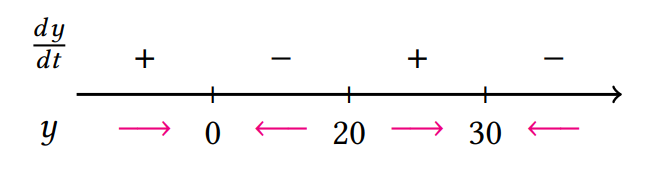
\includegraphics[width=0.9\linewidth]{image/sign-diagram-for-dydt.png}}
        \item Draw the corresponding direction/slope field to judge the stability. For example,\\
        \centerline{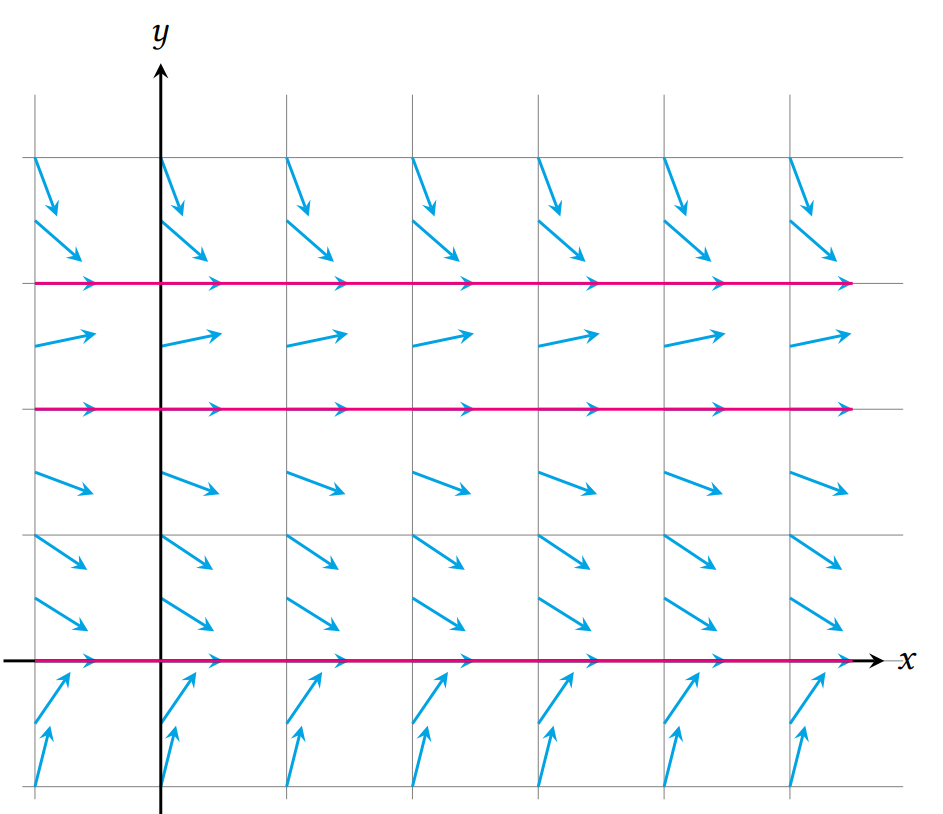
\includegraphics[width=0.5\linewidth]{image/direction-field.png}}
    \end{itemize}
\end{enumerate}
\subsection{Population Dynamics}
\begin{enumerate}
    \item (\textbf{Malthusian model}) It assumes that the rate of change of a population is proportional to its present value. That is $dy/dt=ky\rightarrow y(t)=y_0e^{kt}$, where $y_0=y(0)$. This model suggests that a population would grow exponentially with \textbf{growth rate} k.
    \item (\textbf{Verhulst model}) In Verhulst, our \textbf{growth rate} varies according to the present value $y$ of the population. The formula is given by $\frac{dy}{dt}=[k(1-\frac{y}{y_\infty})]y$, where $dy/dt$ is \textbf{rate of change} and $k(1-y/y_\infty$ is \textbf{growth rate}. This model assumes that a population grows \textbf{logistically}, such that given any initial population, $lim_{t\to \infty}y(t)=y_\infty$
    \item (\textbf{Hunt rate}) Since hunt rate(E) is usually given in constant number per period, and in both models we have rate of change $dy/dt$, so usually we just minus the hunt rate (E) at the right side of our equation. e.g. If hunt rate is 100, $dy/dt=ky-100$
    \item (\textbf{Some useful tips regarding Verhulst model})
    \begin{itemize}
        \item Using basic algebra knowledge, we can see that when $y=y_\infty/2$, the rate of change $dy/dt$ will be maximum.
        \item Given the initial condition $y(0)=y_0$, the solution for Verhulst Model is $y(t)=\frac{y_\infty}{1+(y_\infty/y_0-1)e^{-kt}}$
    \end{itemize}
\end{enumerate}

\section{02. Linear Differential Equation}
\subsection{First-Order Linear Equations}
\begin{enumerate}
    \item (\textbf{First-order Linear Equation}) A \textbf{first-order linear} differential equation is an equation of the form $a(x)y'+b(x)y=c(x)$, with $a(x)\neq 0$. \textbf{First-order} means only have $y'$, cannot have $y'' \cdots$. \textbf{Linear} means the highest order of $y$ must be one, cannot have $y^2 \cdots$. A tip is to treat $y'$ also as a function of $y$, so terms like $y'y$ is also not allowed.
    \item (\textbf{Method of Integrating factor})
    \begin{itemize}
        \item Rewrite the entire equation in standard linear form $y'+p(x)y=q(x)$
        \item Calculate the integrating factor $u=e^{\int p(x)dx}$
        \item Multiply both sides of the equation by $u$: $u(y'+py)=uq\rightarrow (uy)'=uq$
        \item Integrate both sides of the equation. (Remember to add the arbitrary constant $C$ at the right side of the equation at this step!)
    \end{itemize}
    \item (\textbf{Bernoulli differential equation}) It is a diff eq of the form $y'+p(x)y=q(x)y^n\equiv y^{-n}y'+y^{1-n}p(x)=q(x)$. To solve it, use substitution. Substitute $v=y^{1-n}$, so $v'=(1-n)y^{-n}y'$. Then, the Bernouli equation is simply $v'+v(1-n)p(x)=q(x)(1-n)$. Then use integrating factor to solve it.
    \item (\textbf{Some useful substitution}) The sole of substitution is to reduce the equation for first-order linear equation. So, the whole idea is to try some substitution $v$ and find whether $v'$ can help me achieve the goal.
    \begin{itemize}
        \item $v=siny$, $v'=cosy\cdot y'$
    \end{itemize}
\end{enumerate}
\subsection{Higher Order Differential Equation}
In this part, we mainly focus on how to solve homogeneous linear differential equation with constant coefficients.
\begin{enumerate}
    \item (\textbf{Homogeneous/Non-homogeneous}) A \textbf{linear differential equation with constant coefficients} is an equation of the form $a_ny^{(n)}+a_{n-1}y^{(n-1)}+\cdots+a_1y'+a_0y=f(x)$, where $a_i\in R$. When $f(x)=0$, the equation is said to be \textbf{homogeneous}; otherwise, it is said to be \textbf{non-homogeneous}.
    \item (\textbf{Methods to solve homogeneous diff eq with constant coefficients})
    \begin{itemize}
        \item Make a guess $y(x)=e^{\lambda x}$
        \item Plug the guess into the diff eq and form a \textbf{characteristic eqaution}: $a_n\lambda^n+a_{n-1}\lambda^{n-1}+\cdots+a_1\lambda+a_0=0$. Solve for $\lambda$
        \begin{itemize}
            \item If $\lambda \in R$ is a real, distinct root, then a solution is given by $e^{\lambda x}$
            \item If $\lambda \in R$ is a repeated root with multiplicity $\gamma$ (repeats $\gamma$ times), then solutions are obtained by modifying our trial solution by a factor of $x$: $e^{\lambda x}, xe^{\lambda x}, x^2e^{\lambda x},\cdots, x^{r-1}e^{\lambda x}$
            \item If $\lambda, \bar \lambda \in \mathbb{C}$ are conjugate roots $\alpha \pm i\beta$, the solutions $e^{\alpha x}\cos \beta x$, $e^{\alpha x}\sin \beta x$. (Obtained by Euler's formula)
            \item If $\lambda, \bar \lambda \in \mathbb{C}$ are \textit{repeated roots}, the solutions are $e^{\alpha x}\cos \beta x, xe^{\alpha x}\cos \beta x, x^2e^{\alpha x}\cos \beta x, \cdots$ and $e^{\alpha x}\sin \beta x, xe^{\alpha x}\sin \beta x, x^2e^{\alpha x}\sin \beta x, \cdots$
        \end{itemize}
        Note that for an real number order-N equation, the sum of the multiplicity of all its roots must be equal to N.
    \end{itemize}
    \item (\textbf{Superposition Principle}) Let $y_1(x)$ and $y_2(x)$ be solutions to a homogeneous linear differential equation $a_ny^{(n)}+a_{n-1}y^{(n-1)}+\cdots+a_1y'+a_0y=0$. Then a solution to this diff eq is also given by $y(x)=c_1y_1(x)+c_2y_2(x)$, for all $c_1, c_2 \in R$. (This is the general solution)
\end{enumerate}
\end{multicols}

% Dividing Line
\hrulefill \\

\begin{multicols}{3}
\end{multicols}

\end{document}